% ============================================================================
% NOTE TO KAJA / EDUARDO -- read this before the manuscript text below.
% (This note is a LaTeX comment: it will not appear in the compiled PDF.)
%
% This is a first full draft generated directly from the saved result
% dataframes (errors_compact_binsweep.pkl, pca_scores_binsweep.pkl) and the
% real OP maps, using exactly the statistical pipeline described in
% Maps_handover_Kaja.md (uniform-random control, min-over-pairs
% selection-corrected percentile test). All numbers below are computed, not
% invented -- the scripts that produced them are in paper/ and the tables
% behind every number are in paper/tables/.
%
% What this draft IS: parts 1-3 of the handover's suggested paper shape
% (estimation exists and is array-specific -> reproducible across days and
% predicted by oriented-channel count -> the map-carrying PC pair is not
% fixed), plus the EC/EO comparison.
%
% What this draft DELIBERATELY LEAVES OUT: part 4 (orientation-biased
% up-state replay). Per the handover, that analysis needs a new up-state
% detector and a proper non-uniformity test and hasn't been built yet -- I
% did not attempt it rather than fabricate a result. The Moran's-I /
% map-smoothness regression suggested as an explanation for *which* arrays
% are estimated well (handover Sec.5, item 2) is also not included for the same reason:
% it is a new analysis, not a figure the student already produced.
% Author list, funding, and citations are left as placeholders -- I have no
% way to know these. Please treat the Discussion's framing as a starting
% point, not a final scientific judgment: I'm not a domain expert on macaque
% V1 physiology and the interpretive calls (how hard to push each claim,
% what a reviewer will find convincing) deserve your and Eduardo's read.
%
% Data provenance note: params_binsweep.yml points op_map_folder at a
% cluster path (/CSNG/...) that isn't reachable from this machine. I found
% what looks like a local copy at
% ~/work/Eduardo_Fernandez/new_method/monkeys_OP/ and verified it against
% the oriented-channel masks stored in pca_scores_binsweep.pkl -- all
% 1512/1512 (monkey, date, array, condition, bin) cells match exactly, so
% I'm confident it's the right data. Worth a sanity check on your end too
% before submission.
%
% Figures are included below from ../paper/figures/*.pdf (vector, generated
% by paper/fig*.py). Compile with pdflatex from within the paper/ directory:
%   pdflatex draft.tex
% ============================================================================

\documentclass[11pt]{article}

\usepackage[T1]{fontenc}
\usepackage{lmodern}
\usepackage[margin=1in]{geometry}
\usepackage{graphicx}
\usepackage{amsmath}
\usepackage{enumitem}
\usepackage[colorlinks=true,linkcolor=blue,citecolor=blue,urlcolor=blue]{hyperref}
\usepackage[font=small,labelfont=bf]{caption}

\title{Spontaneous population activity reconstructs the orientation-preference
map in a subset of macaque V1 arrays}

% PLACEHOLDER -- fill in the real author list / affiliations / funding.
\author{[Author list placeholder --- Kaja Studekov\'a, Eduardo Fernandez-Lopez,
Karol\'ina Korvasov\'a, et al.]}
\date{}

\begin{document}

\maketitle

\begin{abstract}
Cortical circuits are thought to replay their functional architecture in
spontaneous activity, but whether a fine-grained sensory map can be estimated
from resting-state population activity \emph{alone}, without any
stimulus-evoked reference beyond the map itself, is unclear. We asked whether
the orientation-preference (OP) map of macaque V1, measured with moving-bar
stimulation, can be reconstructed from the correlation structure of
spontaneous multi-unit activity (tMUA) recorded on chronic Utah arrays. For
each array we computed the channel-by-channel correlation matrix during
eyes-closed, eyes-open, and pooled resting-state activity, reduced it with
PCA, and read out each channel's derived orientation from its polar angle in
each pair of principal components, allowing an optimal rotation and mirror
flip against the real map. Significance was assessed against a
uniform-random control (2000 shuffles per array) using a selection-corrected
minimum-over-pairs test, which is markedly stricter than a naive per-pair
test. Across 3 monkeys, 29 arrays, and up to 3 recording days, a subset of
arrays reconstructed the OP map far better than the control (6/29 arrays
were estimated in a majority of their day $\times$ condition cells; 16/29 showed
significant estimation in at least one cell). Estimation was reproducible: the same arrays
(monkey L: arrays 13, 14, 16; monkey N: arrays 1, 6) were estimated on independent
recording days against freshly redrawn controls. Estimation required
sufficient sampling: arrays significant at the 5\% level had systematically
more oriented channels, though the count alone did not guarantee estimation.
The principal-component pair that best carried the map was not fixed across
arrays or conditions, and eyes-closed/eyes-open estimation, while correlated,
diverged in a substantial minority of cases. These results indicate that the
correlation structure of spontaneous V1 activity encodes orientation-map
information that a purely geometric, unsupervised readout can estimate, but
only where the local population is sampled densely enough --- a necessary
constraint for any attempt to infer functional architecture from resting
state alone.
\end{abstract}

\section{Introduction}

\emph{(placeholder --- background on spontaneous activity reflecting the
functional architecture of sensory cortex, prior evidence in visual cortex
(e.g.\ imaging-based work on spontaneous OP-map replay), the specific
novelty here: Utah-array tMUA rather than imaging, a fully
geometric/unsupervised readout, and a selection-corrected significance test.
State the question directly: can PCA on the spontaneous correlation matrix
alone estimate a previously measured OP map, and for which arrays/conditions
does this work?)}

\section{Methods}

\paragraph{Animals and recordings.}
Three macaques (L, N, F) implanted with 64-channel V1 Utah arrays (L: 14
arrays over 3 resting-state recording days; N: 7 arrays over 2 days; F: 8
arrays over 2 days). Each resting-state recording was split into
eyes-closed (EC) and eyes-open (EO) epochs based on an independent eye-state
indicator; results are also reported for the pooled recording (``all'').

\paragraph{Firing-rate matrix.}
Thresholded multi-unit activity (tMUA) at 1~ms resolution was binned into a
firing-rate matrix per channel. Bin size was swept over
$\{20, 50, 100, 250, 500, 750, 1000\}$~ms (Fig.~\ref{fig:S1}); 100~ms gave
the highest fraction of significant cells and was used throughout the main
figures. No binarization or up-state detection was applied to the firing
rate --- this is a deliberate simplification relative to earlier pipelines
in this project.

\paragraph{Channel selection.}
A channel was excluded from the analysis (marked \emph{unoriented}) if its
selectivity index (\texttt{selectivity\_01}) was below 0.15, or if it showed
more than 2 large jumps in its tuning curve (\texttt{num\_f0\_high\_jump >
2}). This selection is applied identically to the real map and to every
control map.

\paragraph{Correlation and PCA.}
For the oriented channels only, we computed the full Pearson correlation
matrix of the firing-rate traces and performed PCA on it (up to 7
components; ``Option A'' --- PCA was not run on the full 64-channel matrix,
which was tried and dropped in favour of restricting to oriented channels).

\paragraph{Geometric OP readout.}
For each of the $\binom{7}{2} = 21$ pairs of principal components, each
channel's polar angle around the centroid of the PC-score cloud was
computed, then rotated ($0$--$360^\circ$, $1^\circ$ steps) and optionally
mirrored to minimize the circular error against the \emph{real} OP map
restricted to oriented channels. This gives one derived OP map per PC pair,
and an error (L1: mean absolute circular error; L2: RMSE circular error)
between the derived and real map.

\paragraph{Control and significance.}
For every array we generated 2000 control OP maps by drawing i.i.d.\
Uniform$[0^\circ, 180^\circ)$ orientations for the oriented channels
(unoriented channels fixed at $-1$), using a deterministic per-array seed.
Because the analysis is free to pick whichever of the 21 PC pairs
reconstructs the map best, a per-pair significance test is optimistically
biased. We therefore used a \textbf{min-over-pairs} test throughout: the
real statistic is the \emph{minimum} error across all 21 pairs, and the
null distribution is built by taking, for \emph{each} control map, its own
minimum error across all 21 pairs. The reported percentile is
$100 \times \text{mean}(\text{null\_min} \le \text{real\_min})$; a
percentile below 5\% means the real reconstruction beats the control after
the multiple-comparison correction. This is substantially stricter than a
naive per-pair test and is the only test used for significance claims in
this paper.

\paragraph{Code and data availability.}
All analysis code (\texttt{functions\_maps.py}, \texttt{compute\_binsweep.py},
\texttt{generate\_controls.py}, \texttt{repack\_binsweep.py}) and parameters
(\texttt{params\_binsweep.yml}) are in the project repository. Figures in
this manuscript were generated by the scripts in \texttt{paper/} from the
saved result tables in \texttt{dataframes/}.

\section{Results}

\subsection{Spontaneous activity estimates the OP map in a subset of arrays}

Figure~\ref{fig:1} shows a representative example (monkey L, array 16): the
measured OP map, the geometric map estimated from the best-performing PC
pair, and the null distribution of the min-over-pairs control statistic.
The real reconstruction (L2 error $= 32.3^\circ$) falls far below the
control distribution (percentile $= 0.35\%$). Panels C and E make the
underlying geometry explicit: the same PC5-vs-PC6 projection of the
spontaneous-activity scores, colored by the measured OP (C) and by the OP
the geometric readout assigns (E) --- panel E is clean by construction (it
\emph{is} the rotation/flip fit), and the question the whole method answers
is how much of that same angular structure panel C already carries.

\begin{figure}[htbp]
  \centering
  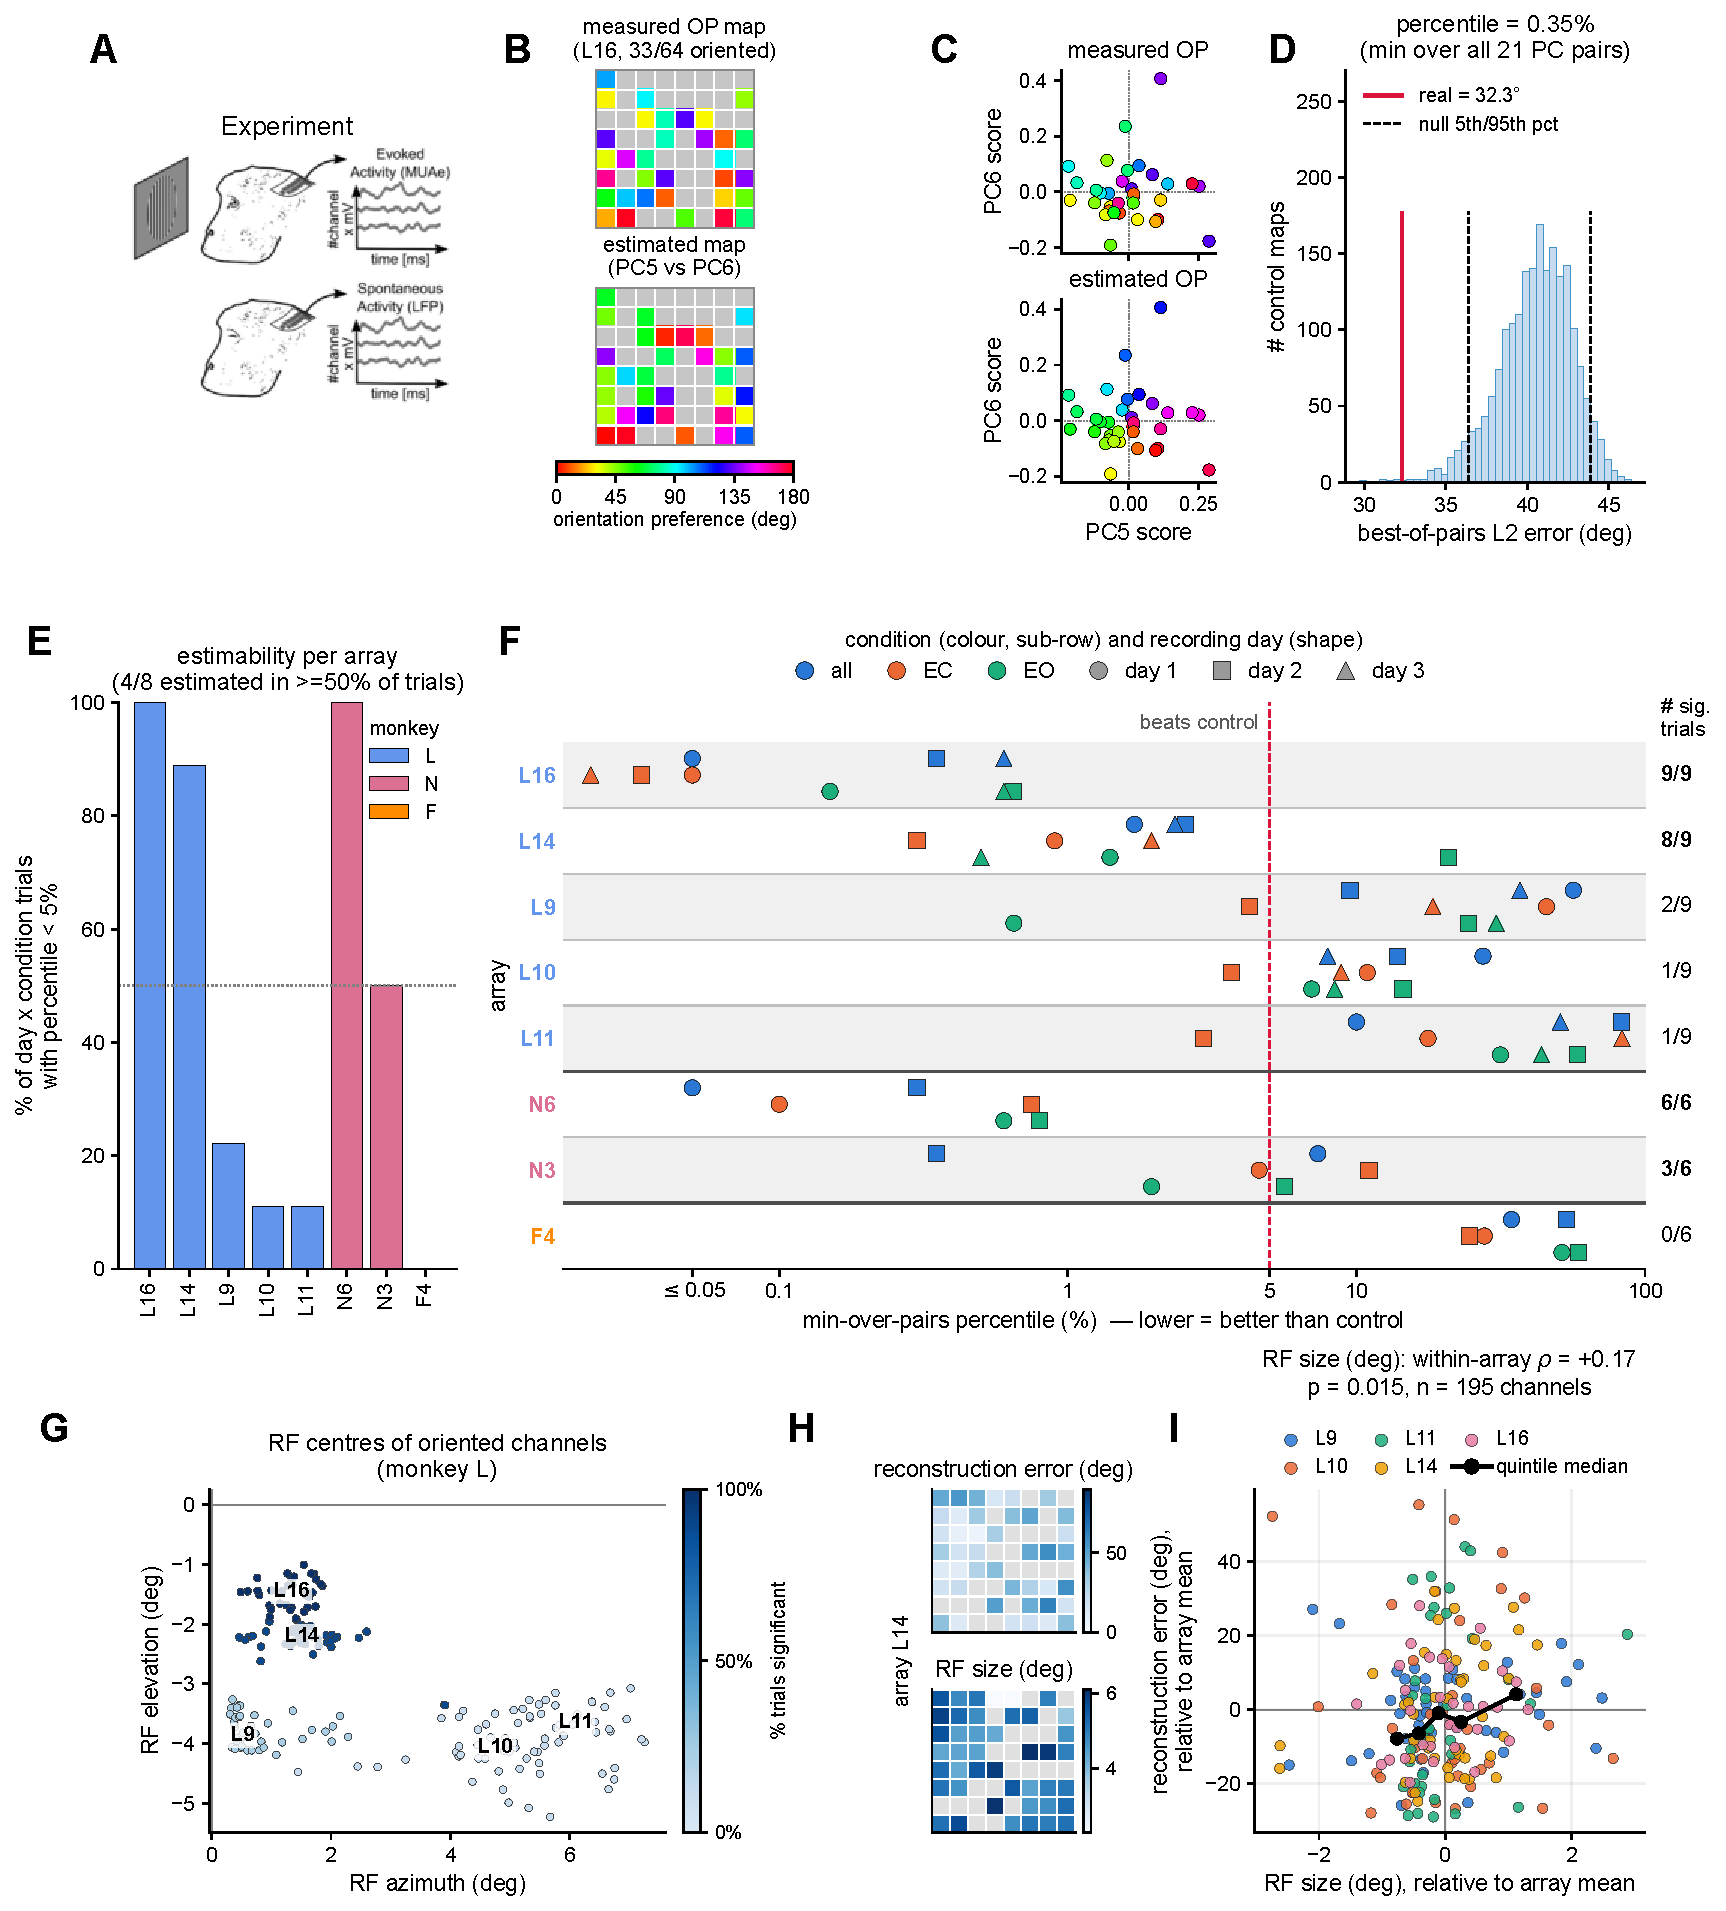
\includegraphics[width=\textwidth]{figures/fig1_example_estimation.pdf}
  \caption{\textbf{Worked example of OP-map estimation, with the underlying
  PC-plane geometry made explicit.} (A) Schematic of the experiment: tMUA is
  recorded from a 64-channel V1 Utah array during spontaneous
  (eyes-closed / eyes-open) activity; a few representative channel traces
  are sketched for illustration. (B) Measured OP map for monkey L, array 16
  (33/64 channels pass the orientation-selectivity criterion; grey =
  excluded). (C) The same oriented channels plotted in the PC5-vs-PC6 plane
  (the best-performing pair for this cell; ``+'' = centroid), colored by
  their \emph{measured} OP. (D) Geometric map estimated from spontaneous
  activity using that PC pair. (E) The same PC-plane coordinates, now
  colored by the \emph{estimated} OP --- the clean radial gradient follows
  directly from the polar-angle rotation/flip fit to panel C. (F) Null
  distribution of the min-over-pairs control statistic (2000 uniform-random
  control maps, each reduced to its own best-of-21-pairs L2 error); the real
  statistic (red) falls at the 0.35th percentile.}
  \label{fig:1}
\end{figure}

This is not a global effect. Figure~\ref{fig:2} shows the min-over-pairs
percentile for every array, averaged across recording days, separately for
the pooled (``all''), eyes-closed, and eyes-open conditions. A subset of
arrays is consistently below the 5\% threshold across all three conditions
--- most clearly L13, L14, and L16, and N1 and N6 --- while others (e.g.\
L4, L6, L15, N2, and every array in monkey F) sit well within the null
range in every condition.

\begin{figure}[htbp]
  \centering
  \includegraphics[width=\textwidth]{figures/fig2_percentile_grids.pdf}
  \caption{\textbf{Estimation is array-specific.} Min-over-pairs percentile
  (uniform-random null; blue $<5\%$ beats control), one grid per monkey,
  rows = array, columns = condition (pooled / eyes-closed / eyes-open),
  averaged across recording days. Bin = 100~ms, L2 norm.}
  \label{fig:2}
\end{figure}

Turning this into a single per-array \textbf{estimability score} --- the
fraction of (day $\times$ condition) cells with percentile $<5\%$ --- makes
the array-specific pattern explicit (Fig.~\ref{fig:3}A): 6 of 29 arrays
are estimated in a majority of their cells (L13, L14, L16, N1, N3, N6), and 16 of
29 arrays (55\%) show at least one significant cell. No array in monkey F
reached the majority-of-cells criterion, although 3 of the 8 F arrays showed
at least one significant cell.

\subsection{Estimation requires enough oriented channels}

Figure~\ref{fig:3}B relates the per-cell percentile to the number of
oriented channels in the array. Significant cells were essentially absent
below roughly 15 oriented channels (10th percentile of oriented-channel
count among significant cells $= 15$), and the fraction of significant
cells rises with channel count across the range sampled here. Channel count
is not sufficient on its own --- several arrays with more oriented channels
than the typical estimable array never reach significance in any cell
(e.g.\ F4, 36 oriented channels; L12, 28 oriented channels; L6, 24 oriented
channels) --- but it is close to necessary: too few oriented channels make
the null and the real distributions indistinguishable regardless of whether
the array's map is, in principle, estimable.

\begin{figure}[htbp]
  \centering
  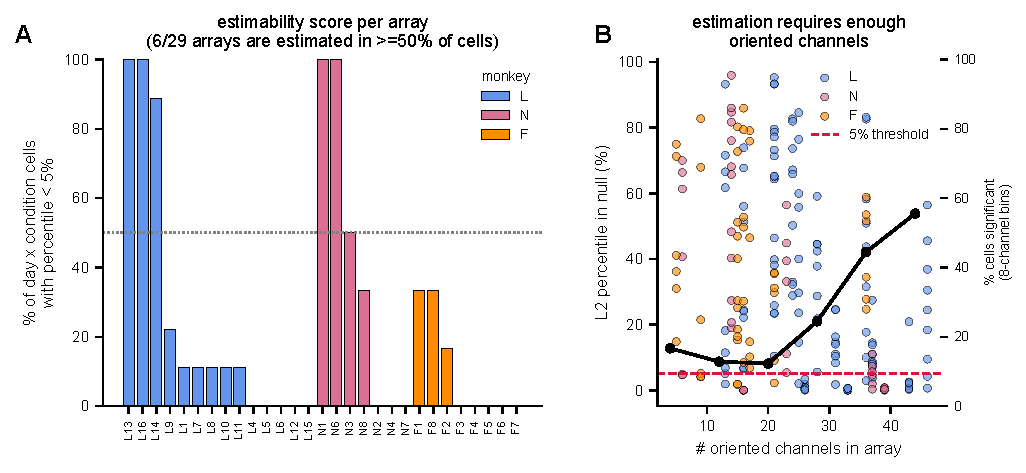
\includegraphics[width=\textwidth]{figures/fig3_estimability.pdf}
  \caption{\textbf{A single estimability score per array, and its
  dependence on oriented-channel count.} (A) Fraction of (day $\times$
  condition) cells per array with percentile $<5\%$, grouped and colored by
  monkey; 6/29 arrays are estimated in a majority of cells. (B) Per-cell
  percentile vs.\ number of oriented channels in the array (colored by
  monkey); overlaid black line: fraction of cells significant within
  8-channel bins of oriented count.}
  \label{fig:3}
\end{figure}

\subsection{Estimation is reproducible across independent recording days}

The single strongest piece of evidence that this is a genuine effect rather
than a selection artifact is that \textbf{the same arrays are estimated well on
different recording days, each with an independently redrawn control}
(Fig.~\ref{fig:2} shows this averaged over days; the per-day grids in
\texttt{paper/tables/} show it is not driven by a single day). Chance
estimation would not be expected to repeat in the same arrays across sessions
collected weeks apart.

Among arrays with enough oriented channels to evaluate reliably ($\ge 25$
oriented channels, condition = all; 12 arrays across the 3 monkeys),
Figure~\ref{fig:4} quantifies how similar the \emph{profile} of which PC
pairs carry information is from day to day: the median L2 distance between
per-pair error profiles was $3.5^\circ$ (L), $3.4^\circ$ (N), and
$2.6^\circ$ (F, $n=1$ array), and the median top-3 winning-pair Jaccard
overlap was 0.20--0.35. With only 3 days for monkey L and 2 for monkeys
N/F, we treat this descriptively rather than claiming a formal significance
level, per the small day count.

Panels C--D of Fig.~\ref{fig:4} make this concrete for two representative,
fully estimable arrays (L13, L16): on every one of the 3 recording days, a
cluster of several PC pairs stays below the 5\% threshold, but the single
best-performing pair (starred) is a different member of that cluster each
day. So day-to-day reproducibility holds at the level of ``the map is
carried by one of a handful of pairs,'' not at the level of a single fixed
pair --- the summary statistics in panels A--B are one way of quantifying
exactly this.

\begin{figure}[htbp]
  \centering
  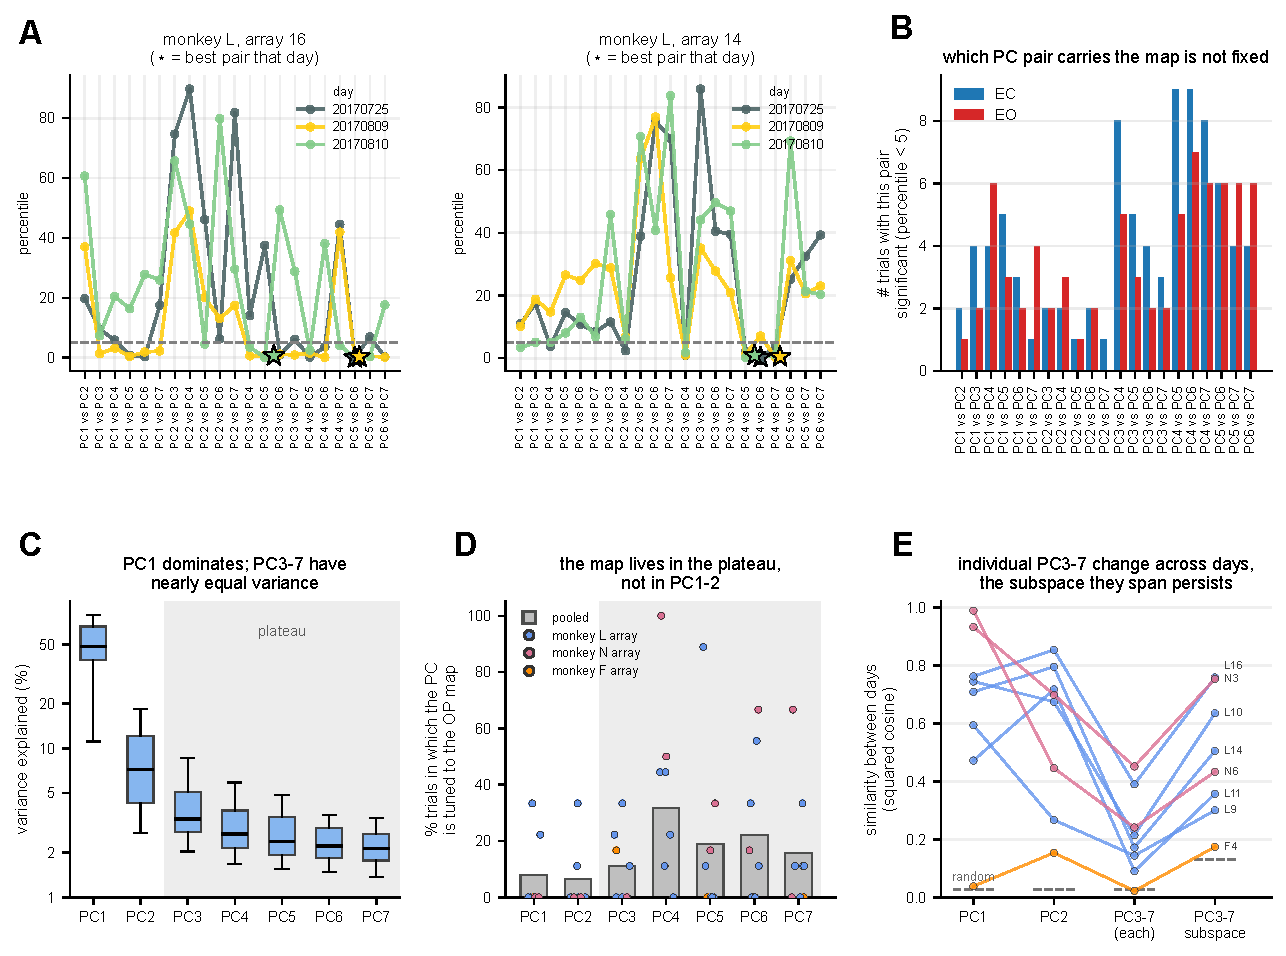
\includegraphics[width=\textwidth]{figures/fig4_day_stability.pdf}
  \caption{\textbf{Day-to-day reproducibility of the map-carrying PC
  pairs}, for arrays with $\ge 25$ oriented channels evaluated on more than
  one recording day. (A) L2 distance between the 21-pair error profile on
  two different days (lower = more similar), pooled across all qualifying
  arrays. (B) Jaccard overlap of the top-3 best-performing pairs between the
  same two days (higher = more similar), pooled across arrays. Black bar =
  median; points = individual day-pairs. (C, D) Concrete per-array
  illustration for two representative, fully estimable example arrays
  (monkey L, arrays 16 and 13): the min-over-pairs percentile of each of the
  21 PC pairs, plotted separately for each of the array's 3 recording days
  (colored lines); the star marks the single best-performing pair on that
  day. A cluster of pairs stays below the 5\% threshold (dashed line) on
  every day, but which specific pair within that cluster wins shifts from
  day to day.}
  \label{fig:4}
\end{figure}

\subsection{The map-carrying principal-component pair is not fixed}

Across the cells that were significant in at least one of EC or EO
($n=23$; Fig.~\ref{fig:5}B), no single PC pair dominates: roughly a third
of the 21 pairs are each significant in 8--10 of the 23 cells, with the
rest spread more thinly. This means the ``readout direction'' through
which orientation information appears in the correlation structure shifts
across arrays, days, and states --- consistent with the hypothesis (to be
tested with a model, see Discussion) that changing input or brain state
rotates which PCs the map loads onto, rather than the map information
disappearing.

\subsection{Eyes-closed vs eyes-open estimation is correlated but not identical}

Figure~\ref{fig:5}A compares the min-over-pairs percentile in EC vs EO for
every array/day with both conditions available ($n=72$ cells). Percentiles
are positively correlated (points cluster around the diagonal), and 14
cells are significant in both conditions. But EC and EO are not
interchangeable: 5 cells were significant in EC only and 4 in EO only ---
a roughly balanced, mixed picture rather than a systematic advantage for
either eye state.

\begin{figure}[htbp]
  \centering
  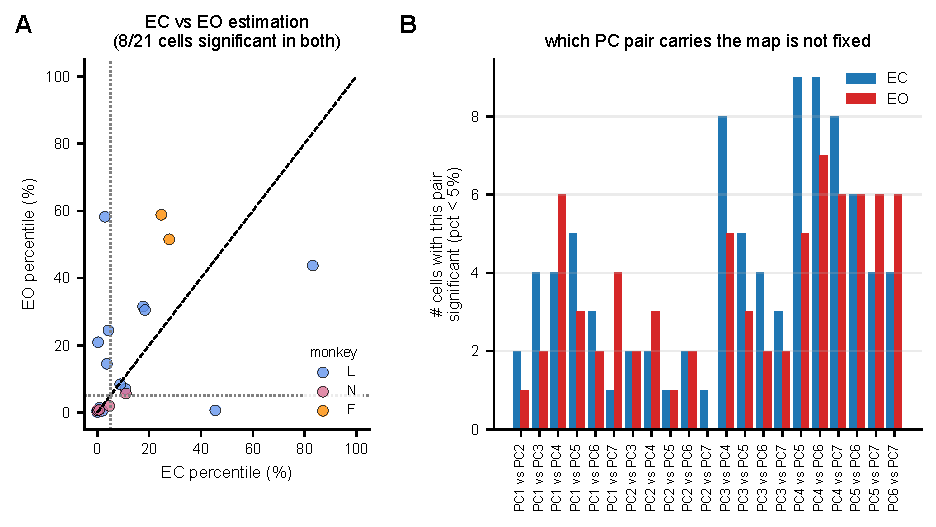
\includegraphics[width=\textwidth]{figures/fig5_eceo_pcpair.pdf}
  \caption{\textbf{Eyes-closed vs.\ eyes-open.} (A) Min-over-pairs
  percentile in EC vs.\ EO for every array/day with both conditions
  available, colored by monkey; dotted lines mark the 5\% threshold. (B)
  Among cells significant in EC and/or EO, the number of cells for which
  each of the 21 PC pairs itself reaches the 5\% per-pair threshold, split
  by condition --- no single pair dominates.}
  \label{fig:5}
\end{figure}

\section{Discussion}

\emph{(placeholder for full discussion --- the following are the
load-bearing points from the handover, to be expanded)}

\begin{itemize}[leftmargin=*]
\item Spontaneous tMUA correlation structure, reduced by PCA and read out
  with a purely geometric procedure, estimates a previously measured sensory
  map in roughly a fifth to a half of V1 arrays (depending on the
  estimability threshold used), established against a uniform-random
  control with a selection-corrected significance test.
\item Estimation is not uniform across arrays, and the arrays that are
  estimated well do so reproducibly across independent recording days ---
  the most defensible part of the finding, because chance estimation would
  not be expected to repeat in the same arrays.
\item The instability of \emph{which} PC pair carries the map
  (Section~3.4) is a natural target for the reviewer objection ``an
  unstable winner is noise.'' The defence used throughout this paper is
  that the null is \emph{also} min-over-pairs (so the correction already
  accounts for the winner moving around within a single array/day), and
  that the estimable arrays are still significant after that correction,
  and reproducibly so across days. A model in which changing input/state
  rotates which PCs the map loads onto (mentioned in the handover as
  reproducible by Katarina's model) would turn this from a weakness into a
  mechanistic result if included in a revision.
\item Two natural next steps, not yet in this draft: (1) regressing the
  per-array estimability score on a spatial-smoothness measure of the
  real OP map (Moran's I) in addition to oriented-channel count, to see
  whether smoothness of the ground-truth map --- not just how many
  channels are oriented --- predicts which arrays are estimated well; (2) the
  up-state replay observation (spontaneous up-states preferentially
  reactivating one orientation), which is preliminary and needs a proper
  up-state detector and a null that accounts for the array's own OP
  composition before it can support a claim.
\end{itemize}

\appendix
\section*{Supplementary figure}
\renewcommand{\thefigure}{S1}
\setcounter{figure}{0}

\begin{figure}[htbp]
  \centering
  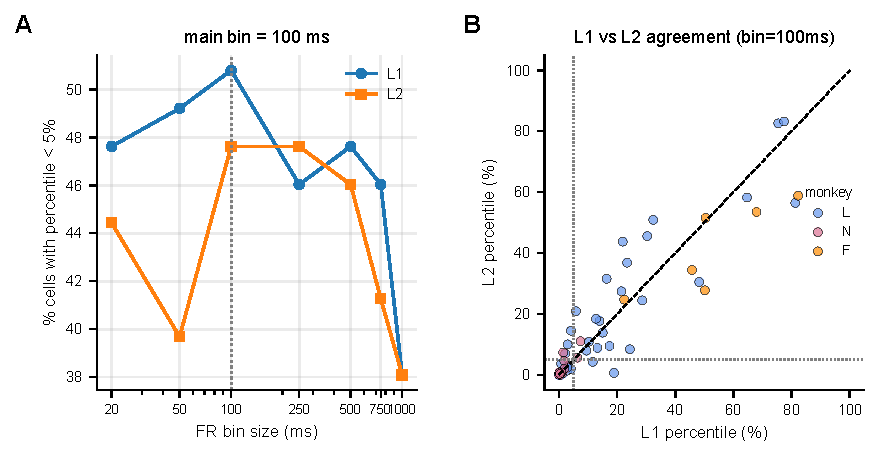
\includegraphics[width=\textwidth]{figures/figS1_bin_sweep.pdf}
  \caption{\textbf{Bin-size and norm robustness.} (A) Fraction of cells
  significant (percentile $<5\%$) as a function of the firing-rate bin size
  used to build the correlation matrix, for both error norms; 100~ms
  (dotted line) was used throughout the main figures. (B) L1 vs.\ L2
  percentile for every cell at the main bin, colored by monkey --- the two
  norms agree closely.}
  \label{fig:S1}
\end{figure}

% PLACEHOLDER -- bibliography. Add a .bib file and \bibliography{refs} here,
% or switch to \usepackage{natbib}/biblatex once citations are added.
% \bibliographystyle{plain}
% \bibliography{refs}

\end{document}
